%===============================================================================
% LaTeX sjabloon voor de bachelorproef toegepaste informatica aan HOGENT
% Meer info op https://github.com/HoGentTIN/bachproef-latex-sjabloon
%===============================================================================

\documentclass{bachproef-tin}

% Titelpagina conform aan HOGENT huisstijl
\usepackage{hogent-thesis-titlepage}
\usepackage{glossaries}
\usepackage{graphicx}
\usepackage{subcaption}
\usepackage{float}
\usepackage{listings}
\usepackage{xcolor}
\usepackage{courier}

\usepackage{tikz}
\usetikzlibrary{shadows}

\definecolor{PigPurple}{RGB}{192, 93, 199}
\lstdefinelanguage{Java}{
    morekeywords={abstract,boolean,break,byte,case,catch,char,class,
        const,continue,default,do,double,else,extends,false,final,
        finally,float,for,goto,if,implements,import,instanceof,int,
        interface,label,long,native,new,null,package,private,protected,
        public,short,static,super,switch,synchronized,this,throw,
        throws,transient,true,try,void,volatile,while,function,render,from
    },
    keywords=[2]{export, return},
    keywordstyle=[2]\color{PigPurple},
    sensitive,
    morecomment=[l]//,
    morecomment=[s]{/*}{*/},
    morestring=[b]",
    morestring=[b]',
}[keywords,comments,strings]

\definecolor{codegreen}{rgb}{0,0.6,0}
\definecolor{codegray}{rgb}{0.5,0.5,0.5}
\definecolor{codepurple}{rgb}{0.58,0,0.82}
\definecolor{backcolour}{rgb}{0.95,0.95,0.92}
\lstdefinestyle{mystyle}{
    language={Java},
    tabsize=2,
    backgroundcolor=\color{backcolour},   
    commentstyle=\color{codegreen},
    keywordstyle=\color{blue},
    numberstyle=\tiny\color{codegray},
    stringstyle=\color{orange},
    basicstyle=\ttfamily\scriptsize,
    breakatwhitespace=false,         
    breaklines=true,                 
    captionpos=b,                    
    keepspaces=true,                 
    numbers=left,                    
    numbersep=5pt,                  
    showspaces=false,                
    showstringspaces=false,
    showtabs=false,                  
    tabsize=2
}

\lstset{style=mystyle}
\renewcommand*{\lstlistingname}{Code fragment}

%%---------- Documenteigenschappen ---------------------------------------------

% De titel van het rapport/bachelorproef
\title{Front end performantie in React-gebaseerde applicaties}

% Je eigen naam
\author{Matthias Tison}

% De naam van je promotor (lector van de opleiding)
\promotor{Leen Vuyge}

% De naam van je co-promotor. Als je promotor ook je opdrachtgever is en je
% dus ook inhoudelijk begeleidt (en enkel dan!), mag je dit leeg laten.
\copromotor{Arvid De Meyer}

% Indien je bachelorproef in opdracht van/in samenwerking met een bedrijf of
% externe organisatie geschreven is, geef je hier de naam. Zoniet laat je dit
% zoals het is.
\instelling{Codifly}

% Academiejaar
\academiejaar{2019-2020}

% Examenperiode
%  - 1e semester = 1e examenperiode => 1
%  - 2e semester = 2e examenperiode => 2
%  - tweede zit  = 3e examenperiode => 3
\examenperiode{1}

% Genereer de `glossaries`
\makeglossaries

%===============================================================================
% Inhoud document
%===============================================================================

\begin{document}

%---------- Taalselectie -------------------------------------------------------
% Als je je bachelorproef in het Engels schrijft, haal dan onderstaande regel
% uit commentaar. Let op: de tekst op de voorkaft blijft in het Nederlands, en
% dat is ook de bedoeling!

%\selectlanguage{english}

%---------- Titelblad ----------------------------------------------------------
\inserttitlepage

%---------- Samenvatting, voorwoord --------------------------------------------
\usechapterimagefalse
\input{voorwoord}
\input{samenvatting}

%---------- Inhoudstafel -------------------------------------------------------
\pagestyle{empty} % Geen hoofding
\tableofcontents  % Voeg de inhoudstafel toe
\cleardoublepage  % Zorg dat volgende hoofstuk op een oneven pagina begint
\pagestyle{fancy} % Zet hoofding opnieuw aan

%---------- Lijst figuren, afkortingen, ... ------------------------------------

% Indien gewenst kan je hier een lijst van figuren/tabellen opgeven. Geef in
% dat geval je figuren/tabellen altijd een korte beschrijving:
%
%  \caption[korte beschrijving]{uitgebreide beschrijving}
%
% De korte beschrijving wordt gebruikt voor deze lijst, de uitgebreide staat bij
% de figuur of tabel zelf.

\listoffigures
\lstlistoflistings
%\listoftables

% Definities van de termen in de `glossary`
\newglossaryentry{kmo}{name=KMO, description={Kleine of Middelgrote Onderneming}}
\newglossaryentry{html}{name=HTML, description={HyperText Markup Language}}
\newglossaryentry{css}{name=CSS, description={Cascading Style Sheet}}
\newglossaryentry{ajax}{name=AJAX, description={Asynchronous JavaScript And HTML}}
\newglossaryentry{js}{name=JS, description={javaScript}}
\newglossaryentry{dom}{name=DOM, description={Document Object Model}}
\newglossaryentry{seo}{name=SEO, description={Search Engine Optimization}}
\newglossaryentry{ux}{name=UX, description={User eXperience}}
\newglossaryentry{ui}{name=UI, description={User Interface}}
\newglossaryentry{ecma}{name=ECMA, description={European Computer Manufacturers Association}}
\newglossaryentry{mvc}{name=MVC, description={Model View Controller}}
\newglossaryentry{jsx}{name=JSX, description={JavaScript eXtension}}
\newglossaryentry{api}{name=API, description={Application Programming Interface}}
\newglossaryentry{www}{name=WWW, description={World Wide Web}}
\newglossaryentry{fps}{name=fps, description={Frames per second}}
\newglossaryentry{cpu}{name=cpu, description={Central processing unit}}

% Print alle termen in de `glossary`
\printglossaries

% Als je een lijst van afkortingen of termen wil toevoegen, dan hoort die
% hier thuis. Gebruik bijvoorbeeld de ``glossaries'' package.
% https://www.overleaf.com/learn/latex/Glossaries

%---------- Kern ---------------------------------------------------------------

% De eerste hoofdstukken van een bachelorproef zijn meestal een inleiding op
% het onderwerp, literatuurstudie en verantwoording methodologie.
% Aarzel niet om een meer beschrijvende titel aan deze hoofstukken te geven of
% om bijvoorbeeld de inleiding en/of stand van zaken over meerdere hoofdstukken
% te verspreiden!

\input{inleiding}
\input{react}

%=======================================================================
% Theoretische perfromantie hoofdstuk
%=======================================================================

\chapter{\IfLanguageName{dutch}{Theoretische performantie}{Theoretic performance}}
\label{ch:theoretischePerformantie}

\section{\IfLanguageName{dutch}{Metingen zijn belangrijk}{Measurements are important}}
\label{sec:importantMetrics}

Metingen zijn de basis waarop optimalisaties worden uitgevoerd, dit is in het geval van performantie niet anders. Weten waar werkpunten liggen en op basis daarvan een plan van aanpak opstellen zorgt voor doelgerichte optimalisatie. Arbitrair verandering aanbrengen zonder een duidelijke kijk te hebben op wat noodzakelijk is stelt zichzelf in vraag.

\subsection{\IfLanguageName{dutch}{De grootste factor}{The biggest factor}}
\label{sec:biggestFactor}

In de sectie~\ref{sec:whyPerformance} op pagina~\pageref{sec:whyPerformance} werd er al nadruk gelegd op de impact die een slechte performantie kan achterlaten voor een bedrijf, maar wat de gebruiker vindt geeft het uiteindelijke verdict. Waar het om draait voor de hedendaagse gebruiker van het \gls{www} is snelheid. Gebruikers willen zoveel mogelijk informatie op hun beeld krijgen op een snelle en efficiënte manier. \\
In het artikel van~\textcite{Everts2016} werden conclusies getrokken uit Google Analytics en data van derde partijen die vrijwillig bereid waren hun specifieke data te delen. De conclusies waren unaniem, te lange laadtijd zorgt voor ontevredenheid bij de gebruiker. Trage sites (19 seconden laadtijd) hebben zeer korte gebruikerssessies en vervolgens ook een hoger debouncepercentage, waarbij snelle sites (5 seconden laadtijd) 70 procent langere gebruikerssessies en 35 procent minder debouncepercentage ondervinden.

\subsection{\IfLanguageName{dutch}{Metrieken}{Metrics}}
\label{sec:metrics}

Wat zij de metrieken waarmee rekening gehouden worden in welzijn van de gebruiker? Dit kan gaan van hoe snel de eerste pixels op het scherm verschijnen tot de reactietijd van een interactie die de gebruiker uitvoert.

\subsubsection{\IfLanguageName{dutch}{FCP (First Contentful Paint)}{FCP (First Contentful Paint)}}
\label{sec:fcp}

De tijd totdat een gebruiker iets visueel op het scherm te zien krijgt wordt is the frist contentful paint. Het is een maatstaf om een idee te geven wanneer de gebruiker voor het eerst inhoud zal te zien krijgen die hij of zij kan consumeren. 

\subsubsection{\IfLanguageName{dutch}{FMP (First Meaningful Paint)}{FCP (First Meaningful Paint)}}
\label{sec:fmp}

In aanvulling op een first contentful paint wordt ook rekening gehouden met de tijd tot het eerste deel van de website waar een gebruiker iets aan heeft, deze belangrijke delen van een website worden hero elementen genoemd. In tegenstelling tot first contentful, wat nog maar een enkel woord kan zijn dat op het scherm verschijnt, is the first meaningful veel verfijnder. Wanneer een gebruiker het belangrijkste deel van een website eerst te zien krijgt aan een verwachte snelheid zal er minder aandacht geschonken worden wanneer de rest van diezelfde pagina verschijnt. Waardoor een website veel sneller oogt.

\subsubsection{\IfLanguageName{dutch}{Interactie}{Interaction}}
\label{sec:interaction}

Interactie is een algemeen begrip en wordt onderverdeeld in verschillende criteria. Met het steeds sneller evolueren van de niche, dat het internet is, worden doelstelling opgelegd die de industrie verwacht behaald te zien. \\ 
In figuur~\ref{fig:InteractionSpeedTarget} op pagina~\pageref{fig:InteractionSpeedTarget} worden de doelstellingen in verband met interactie aangekaart, bron van deze informatie komt is het artikel van~\textcite{Taub2017}.

\begin{itemize}[label={}]
    \item \textbf{Time to interact}:
    Geeft een indicatie weer van de tijd die nodig is vooraleer de gebruiker interactie kan voeren met delen van de website, zoals bv. een input veld selecteren, doorklikken op een link, animaties starten,\dots \newline
    \item \textbf{Interaction frame rate}:
    Meeste schermen hebben een refresh snelheid van 60\gls{fps}, wanneer er onder 60 wordt gegaan kan dit snel aanzien worden als \textit{laggy} voor een gebruiker. De oorzaak hiervoor is vaak teveel schrijven/lezen of een verrommeling van het \gls{dom}. \newline
    \item \textbf{Interaction response time}:
    Een abstracte maatstaf voor de snelheid waarmee een interactie word waargenomen door de gebruiker. Hoe lager deze waarde ligt, hoe sneller een website zal waargenomen worden.
\end{itemize}

\begin{figure}[H]
    \tikz\node [drop shadow={
        shadow scale=0.98,
        shadow xshift=0ex,
        shadow yshift=0ex,
        opacity=0.1,
    }]
    {\fcolorbox{black}{white}{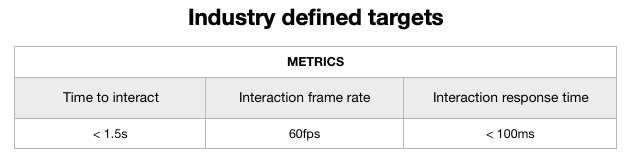
\includegraphics[width=\linewidth]{InteractionSpeedTarget}}};
    \caption{Verwachte waarden opgelegd door de industrie}
    \label{fig:InteractionSpeedTarget}
\end{figure}

\subsubsection{\IfLanguageName{dutch}{Laadproces}{Loading process}}
\label{sec:loadingProcess}

Wanneer een website wordt geladen worden er een bepaald aantal fasen doorlopen vooraleer de eerste pagina op het scherm tevoorschijn kan komen. In figuur~\ref{fig:browserPageLoadTimeline} op pagina~\pageref{fig:browserPageLoadTimeline} worden de fasen aangetoond op een as doorheen de tijd. Voor deze scriptie ligt de focus op frontend tijd.

\begin{itemize}[label={}]
    \item \textbf{\gls{dom} processing}:
    Na het verkrijgen van de \gls{html}, die via requests van de server werd gehaald, wordt deze omgezet naar een \gls{dom}. \newline
    \item \textbf{Pagina rendering}:
    Wanneer het \gls{dom} is aangemaakt begint de browser met het renderen van de pagina op basis van het \gls{dom}. In deze fase wordt de inhoud verwerkt en nadien kan de browser het window load event initialiseren.
\end{itemize}

\begin{figure}[h!]
    \tikz\node [drop shadow={
        shadow scale=0.98,
        shadow xshift=0ex,
        shadow yshift=0ex,
        opacity=0.2,
    }]
    {\fcolorbox{black}{white}{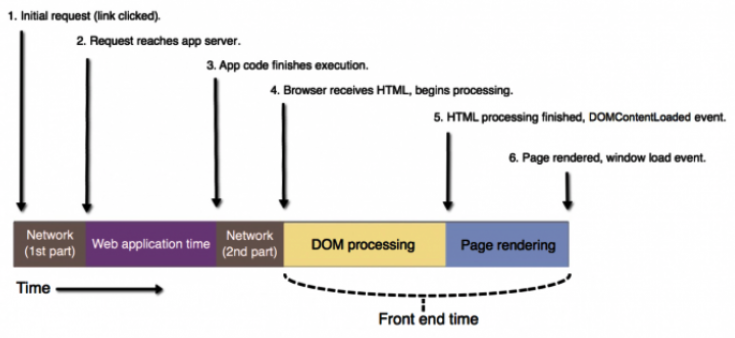
\includegraphics[width=\linewidth]{BrowserPageLoadTimeline.png}}};
    \caption{Tijdlijn voor het laden van een pagina, Bron:~\textcite{Relic2016}}
    \label{fig:browserPageLoadTimeline}
\end{figure}

\subsection{\IfLanguageName{dutch}{Tools}{Tools}}
\label{sec:testTools}

Zoals voordien al aangegeven in sectie~\ref{sec:biggestFactor} op pagina~\pageref{sec:biggestFactor} is snelheid alles bepalend en dit is te meten op basis van verschillende metrieken, welke al reeds besproken werden in sectie~\ref{sec:metrics} op pagina~\pageref{sec:metrics}. Voor het daadwerkelijk meten van deze maatstaven zijn er verschillende tools op de markt. Zo zijn er tools voor performantie tests manueel of geautomatiseerd kunnen zijn. Ook de Chrome DevTools bieden een geïntegreerde tool voor het testen van performantie. Hieronder enkele bekende voorbeelden van dergelijke tools: \\

\begin{itemize}[label={}]
    \item \textbf{MachMetrics}:
    Een tool die geautomatiseerde testresultaten voor snelheid dagelijks opmaakt en doorstuurt. Het is een best practice om de statistieken van je website op gepaste tijdstippen te analyseren. Het internet en daarbij ook websites zijn in continue verandering. \newline
    \item \textbf{WebPageTest}:
    Online platform voor het testen van allround performantie in verschillende browsers op populaire besturingssystemen.  \newline
    \item \textbf{Lighthouse}:
    Open-source tool geïntegreerd in Chrome DevTools, maar kan ook als node module of in command line uitgevoerd worden. De tool stelt verschillende audits ter beschikking om de kwaliteit van websites na te gaan. Het genereert rapporten voor de prestaties van uitgevoerde audits.
\end{itemize}

\chapter{\IfLanguageName{dutch}{Praktische performantie}{Practical performance}}
\label{ch:praktischePerformantie}

%=======================================================================
% Technische perfromantie hoofdstuk
%=======================================================================

React biedt talloze oplossing voor het bevorderen van performantie, om een kijk te krijgen op enkele van de meest courante technieken wordt er in dit hoofdstuk een overzicht opgesteld. Enkele van de oplossingen die worden aangehaald zijn nagebootst binnen een testomgeving, waarna de resultaten worden geanalyseerd. Neem op voorhand aan dat dit niet de enige mogelijkheden zijn voor het optimaliseren van performantie. De voorgestelde technieken zijn onderverdeeld in 3 categorieën: \\

\begin{itemize}[label={}]
    \item \textbf{Native}:
    De oplossingen die React ons zelf bied als zijnde deel van de core functionaliteiten \newline
    \item \textbf{Framework}:
    Mogelijkheden die we specifiek kunnen toepassen door het gebruik van React  \newline
    \item \textbf{Tools}:
    Functionaliteiten afkomstig van een derde partij die we kunnen integreren in de codebase
\end{itemize}

\section{\IfLanguageName{dutch}{Native}{Native}}
\label{sec:nativeOplossingen}

Door React in scope te plaatsen is er toegang tot de React top-level \gls{api}. Zoals wordt aangegeven in figuur~\ref{fig:reactImport} op pagina~\pageref{fig:reactImport} is de import het aanspreekpunt voor de \gls{api} en maakt alle React functionaliteiten aanspreekbaar. Zoals wordt aangegeven in figuur~\ref{fig:reactImport} op pagina~\pageref{fig:reactImport}.

\begin{figure}[H]
    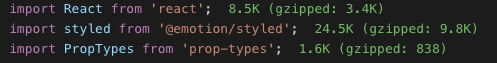
\includegraphics[width=\linewidth]{ReactInScope.png}
    \caption{React in scope}
    \label{fig:reactImport}
\end{figure}

\subsection{\IfLanguageName{dutch}{Gebruiken van de Fragment tag}{Usage of the Fragment tag}}
\label{sec:fragmentsPraktisch}

Een probleem dat vaak voorkomt wanneer het gaat om performantie is het lezen en schrijven naar het \gls{dom}. \gls{dom} manipulaties zijn op zich zeer belastend en vragen veel \gls{cpu}-tijd. Als het \gls{dom} vol wordt gestoken met nestingen van nodes ontstaat er vanzelfsprekend vertraging.\\
In sectie~\ref{sec:fragments} op pagina~\pageref{sec:fragments} werd uitgelegd hoe React fragments het \gls{dom} vrijhouden van een overrompeling aan nutteloze tags, waaronder vooral <div> tags.

\subsection{\IfLanguageName{dutch}{Extenden van React.PureComponent}{Extend of React.PureComponent}}
\label{sec:pureComponent}

Pure component is exact hetzelfde als een gewoon component in React. Het verschil tussen beiden ligt bij het aanroepen van de lifecycle methode shouldComponentUpdate(), die op een andere manier uitgevoerd wordt. Bij een normaal component zal er altijd een re-render uitgevoerd worden wanneer er iets aan props of state veranderd. In een pure component wordt er in de shouldComponentUpdate functie aan shallow comparison gedaan van props en state.\\
Bij shallow comparison worden de waarden en referenties van de vorige props en state vergeleken met de volgende. Deze controle is goedkoop, zeker in vergelijking met het telkens re-renderen van een component. Het nadeel is dat er geen controle wordt gedaan voor de waarden in geneste objecten. \\
Het omzetten gaat ervoor zorgen dat er minder re-renders gebeuren. Dit wordt ook overgedragen naar de kinderen van een pure component, daardoor is het af te raden voor componenten met kinderen, tenzij al deze ook pure components worden.\\
Het is een best practice om een gewoon klasse component om te zetten wanneer het eenvoudige state en props bevat. Het gebruik van een pure component geeft een performantie boost zonder dat er veel aanpassingen moeten worden gedaan aan de initiële code.\\
Figuur~\ref{fig:extendPureComponent} op pagina~\pageref{fig:extendPureComponent} geeft aan waar de aanpassing plaats vindt.

\begin{figure}[H]
    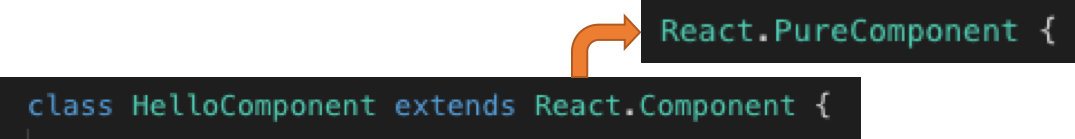
\includegraphics[width=\linewidth]{ExtendPureComponent.png}
    \caption{Veranderen van component naar pure component}
    \label{fig:extendPureComponent}
\end{figure}

%\subsubsection{\IfLanguageName{dutch}{Experiment}{Experiment}}
%\label{sec:pureComponentExp}


\subsection{\IfLanguageName{dutch}{Wikkelen in React.Memo}{Wrap in React.Memo}}
\label{sec:memo}

Memoization is een techniek voor het optimaliseren van snelheid in computer programma's. Door de dure functies, die regelmatig worden uitgevoerd, op te slaan in het cache geheugen kunnen ze veel sneller uitgevoerd worden in de toekomst. React memo werkt volgens hetzelfde principe.\\
React Memo is gelijkaardig aan het extenden van een pure component, het geeft controle over het renderen van functionele componenten. Als een functioneel component wordt gewikkeld in React.memo() worden bij elke re-render enkel de \gls{ui}-elementen opnieuw gerenderd die geüpdatet props nodig hebben.

\subsection{\IfLanguageName{dutch}{React lazy}{React lazy}}
\label{sec:lazy}

Het integreren van code-splitting helpt voor het lazy loaden van componenten. Alles tegelijk in één keer downloaden voor het inladen van de pagina is niet optimaal. \gls{ui} elementen worden ingeladen zonder dat er ooit interactie is met de gebruiker. Tijdens lazy loading wordt gewacht om code in te laden tot wanneer het wel degelijk nodig is.\\
Figuur~\ref{fig:lazyLoading} op pagina~\pageref{fig:lazyLoading} toont een voorbeeld voor het lazy loaden van een component.

\begin{lstlisting}[caption=Lazy loading a component, label={fig:lazyLoading}]
    // MyComponent.js
    class MyComponent extends Component{
        render() {
            return (<div>MyComponent</div>);
        }
    }
    
    // App.js
    import React from 'react';
    
    const MyComponent = React.lazy(()=>import('./MyComponent.js'))
        function AppComponent() {
            return (
                <div>
                    <MyComponent />
                </div>
            );
    }
\end{lstlisting}

\subsubsection{\IfLanguageName{dutch}{Suspense}{Suspense}}
\label{sec:suspens}

Suspense is een concept dat werd geïntroduceerd met de komst van React lazy in React versie 16.6. Het bied een fallback functie voor componenten die lazy loaded zijn. Tijdens het dynamisch inladen van een component kan er een laad tijd ontstaan afhankelijk van de document grootte. Figuur~\ref{fig:suspenseLazy} op pagina~\pageref{fig:suspenseLazy} geeft aan hoe die laadtijd wordt opgevangen met suspense.\\

\newpage
\begin{lstlisting}[caption=Lazy loading met suspense, label={fig:suspenseLazy}]
    // MyComponent.js
    class MyComponent extends Component{
        render() {
            return (<div>MyComponent</div>);
        }
    }
    
    // App.js
    import React, { Suspense } from 'react';
    
    const MyComponent = React.lazy(()=> import('./MyComponent.js'));
    function AppComponent() {
        return (
            <Suspense fallback={<div>Loading ...</div>} >
                <MyComponent />
            </Suspense>
        );
    }
\end{lstlisting}

\section{\IfLanguageName{dutch}{Framework}{Framework}}
\label{sec:frameworkOplossingen}

\subsection{\IfLanguageName{dutch}{Propagatie}{Propagation}}
\label{sec:propagatie}

Bij propagatie geven we properties mee aan een component, om het een bepaalde vorm te geven aan het deel van de \gls{ui} die geretourneerd wordt. In praktijk is het mogelijk om alle props die een ouder bezit door te geven aan zijn kinderen door alle props te spreaden in de component tag. Sectie~\ref{sec:spreadOperator} op pagina~\pageref{sec:spreadOperator} geeft aan hoe de spread operator functioneert en hoe props worden gespread in een component.\\
Het spreaden van het volledige prop object in de component tag is niet altijd een best practice. Wanneer het props object exact de gewenste waarden bevat om door te geven aan een volgend component is er geen probleem. Als er geen zekerheid is over de inhoud van het props object is het een bad practice om deze te spreaden. Door het doorsturen van een inhoudelijk onbekend props object is er grote kans dat we het \gls{dom} vervuilen door properties zonder afhankelijkheid toe te kennen aan componenten.

\subsection{\IfLanguageName{dutch}{Function calls in de render functie}{Function calls in the render function}}
\label{sec:functionCalls}

Figuur~\ref{fig:funcCalls} op pagina~\pageref{fig:funcCalls} toont twee voorbeelden voor het uitvoeren van een functie binnen in de render functie van een component. Het eerste voorbeeld zal telkens een nieuwe referentie aanmaken voor de functie wanneer hij opnieuw gerenderd wordt. Constant nieuwe referenties aanmaken is een bad practice in het performance handboek.\\
Voor het tegengaan van het steeds opnieuw aanmaken van een referentie maken we een arrow functie aan buiten de render. Wanneer de functie nu wordt aangeroepen wordt de referentie naar de arrow functie bewaard.

\newpage
\begin{lstlisting}[caption=Lazy loading met suspense, label={fig:funcCalls}]
     // Functie uitvoeren in de render fucntie
     class MyComponent extends React.Component {
        render() {
            return (
                <button onClick={() => { console.log('Hey, you clicked!'); }}>Click me!</button>
            );
        }
    }
    
    // Functie uitvoeren buiten de render functie
    class MyComponent extends React.Component {
        const handleClick = () => {
            console.log('Hey, you clicked!');
        }
        
        render() {
            return (
                <button onClick={this.handleClick}>Click me!</button>
            );
        }
    }
\end{lstlisting}

            

%%=============================================================================
%% Conclusie
%%=============================================================================

\chapter{Conclusie}
\label{ch:conclusie}

% TODO: Trek een duidelijke conclusie, in de vorm van een antwoord op de
% onderzoeksvra(a)g(en). Wat was jouw bijdrage aan het onderzoeksdomein en
% hoe biedt dit meerwaarde aan het vakgebied/doelgroep? 
% Reflecteer kritisch over het resultaat. In Engelse teksten wordt deze sectie
% ``Discussion'' genoemd. Had je deze uitkomst verwacht? Zijn er zaken die nog
% niet duidelijk zijn?
% Heeft het onderzoek geleid tot nieuwe vragen die uitnodigen tot verder 
% onderzoek?

Uit het onderzoek dat gevoerd is kunnen we concluderen dat er wel degelijk vele technieken bestaan voor het verbeteren van de frontend performantie. Er zijn oplossingen die niet van het framework zelf komen, maar van een derde partij zoals bepaalde libraries.\\
Het is een goede zaak om een overzicht te hebben van optimalisatie technieken voor een specifiek framework, hier in dit geval React. Waar het onderzoek wat vast loopt is het uitdagen van de reeds bestaande technieken. Alle mogelijke optimalisaties zijn reeds uitgevoerd en onderzocht en om een onderzoek te voeren die werkelijk performantie gaat optimaliseren op een innovatieve manier is een proces van maanden. \\
Deze scriptie is wel een leidraad voor developers die beginnen met React voor hun frontend uitwerkingen. Er kunnen lessen getrokken worden uit het gevoerde onderzoek en zorgen voor een optimaal gebruik van het framework vanaf het begin. 



%%=============================================================================
%% Bijlagen
%%=============================================================================

\appendix
\renewcommand{\chaptername}{Appendix}

%%---------- Onderzoeksvoorstel -----------------------------------------------

\chapter{Onderzoeksvoorstel}

Het onderwerp van deze bachelorproef is gebaseerd op een onderzoeksvoorstel dat vooraf werd beoordeeld door de promotor. Dat voorstel is opgenomen in deze bijlage.

% Verwijzing naar het bestand met de inhoud van het onderzoeksvoorstel
%---------- Inleiding ---------------------------------------------------------

\section{Introductie} % The \section*{} command stops section numbering
\label{sec:introductie}

Performantie is voor een bedrijf dat zich specialiseert in web- en native applicaties een absoluut werkpunt bij elk project dat ze aangaan. Dit wordt nog groter wanneer het gaat over complexe applicaties. Codifly is een start-up en specialiseert zich net op dit gebied. Het heeft er alle baad bij een grondig onderzoek naar performantie te doen binnen het framework waar ze hun applicaties op baseren, dit zijnde React.

Voor een bedrijf als Codifly is het belangrijk om consistent sterke, nauwkeurige, dynamische en vooral performante producten aan hun klanten af te kunnen leveren. Om dit niveau van applicaties te kunnen garanderen is het belangrijk om grondig onderzoek te doen.
Een specifiek, maar toch breed onderzoek, waar we ons afvragen: Hoe meten we de performantie binnen het framework? Welke effecten hebben diverse performantie verbetering methoden? Kunnen meerdere methoden gecombineerd worden? Hoe herwerken we onze React codebase hiernaar? Zijn er bepaalde 'regels' te hanteren? Zoja, welke regels moeten gehanteerd worden? Bestaan er specifieke technologieën? ...

%---------- Stand van zaken ---------------------------------------------------

\section{State-of-the-art}
\label{sec:state-of-the-art}

De performantie binnen React gebaseerde applicaties is goed ontvangen door de meeste developers toen het bijna 3 jaar geleden op de voorgrond kwam. Het is nog steeds een veel gebruikt framework om sterke en complexe applicaties te maken, zowel web als native. Aangezien React een steeds verder uitbouwend framework is, zijn onderzoeken naar performantie binnen React meer dan een must. 

Een 3 jaar terug deed ~\textcite{DeCock2016} aan de HoGent een soortgelijke studie, daar noemde hij React een moderne webtechnologie. In het betreffende onderzoek kwam hij tot de conclusie dat het een verfrissend concept is, maar nog niet helemaal op punt staat voor fulltime developers. Nu, na de goede opkomst van React over de voorbije jaren, wordt in deze studie nieuw onderzoek gedaan en analyseert het de vorderingen van het framework.

Er werden al reeds performantie onderzoeken uitgevoerd in React, maar het zijn telkens vergelijkende studies. Deze proberen aan te tonen waarom React, of het andere onderzochte framework, beter zou zijn in bepaalde situaties. Een echt onderzoek naar hoe zwakke performantie aan te pakken, of simpel weg te verbeteren, binnen React zelf wordt niet gedaan. Hierin onderscheid het onderzoek zich van de rest. De studie neemt het probleem concreet aan binnen React.


%---------- Methodologie ------------------------------------------------------
\section{Methodologie}
\label{sec:methodologie}

Het onderzoek dat wordt uitgevoerd ligt in de loop met de projecten die worden aangegaan binnen de stage. Stage vindt plaats in het hierboven vernoemde stagebedrijf Codifly. De verschillende experimenten die worden uitgevoerd zijn gebaseerd op eigen test applicaties en projecten waar aan bijgedragen wordt binnen het bedrijf. Door observaties, studies en experimenten te doen naar verschillende aspecten binnen React performantie kunnen er antwoorden geformuleerd worden op aangehaalde vragen.

Om de performantie te meten bestaan er tools binnen React zelf, zoals 'react-benchmark' die aangewezen werd door de co-promotor. Er is ook een performance tool ingebouwd in React zelf. Simulaties voor kleine testen worden uitgevoerd op zelf ontwikkelde test applicatie. 

%---------- Verwachte resultaten ----------------------------------------------
\section{Verwachte resultaten}
\label{sec:verwachte_resultaten}

Een optimalisatie van de codebase die zorgt voor een verbetering van de performantie. Waarbij het hanteren van de methoden een positieve invloed hebben op het optimaliseren van laadtijden, minimaliseren van bundle sizes, code splitting, ...

De resultaten zorgen voor een betere aanpak en sterke basis voor consistente performantie in toekomstige projecten.

%---------- Verwachte conclusies ----------------------------------------------
\section{Verwachte conclusies}
\label{sec:verwachte_conclusies}

React is een volwaardig framework dat een goed gebalanceerde performantie biedt voor het bouwen van stabiele en complexe web- en native applicaties. Een framework waar performantie kan verbeterd worden met de juiste hanteringen.




%%---------- Referentielijst --------------------------------------------------

\printbibliography[heading=bibintoc]

\end{document}
